\chapter{User experience example}\label{app:user_experience}
\section{Tomato ketchup bottle}
Around 1889 Heinz introduced its octagonal glass ketchup bottle. The iconic glass bottle was their staple for over a hundred years. But in the world of user experience research not the glass bottle, but the current plastic bottle is known as one of the greatest innovations since the invention of semiconductors. (\textit{slightly exaggerated})

\subsection{Innovations}
Although Heinz had no intention to reinvent their ketchup bottle, it was determined to better understand how people were consuming its ketchup at home. 
The company did an extensive market-research in which researchers visited ordinary families and watched the way they used their ketchup. Something remarkable happened. Something that probably exceeded their greatest expectations.

Casey Keller, who was the chief growth offer for Heinz at the time, said: 

\begin{displayquote}
    \textit{
    "I remember sitting in one of those households, There was a three-year-old and a six-year-old, and what happened was that the kids asked for ketchup and Mom brought it out. It was a forty-ounce bottle. And the three-year-old went to grab it himself, and Mom intercepted the bottle and said, 'No you are not going to do that.' She physically took the bottle away and doled out a little dollop. You could see that the whole thing was a bummer."}
    \cite{Gladwell2009}
\end{displayquote}

Researchers had already discovered that children consume approximately 60\% more ketchup than an adult. But now, they found out that their biggest consumers, children, did not have direct access to the bottle. For as long as the parents are in control they would always restrain the consumption levels. 

The result was a so called 'EZ Squirt bottle'. This is a bottle completely made out of plastic with a cone-shaped tip. After thoroughly analysing the families that used this new bottle, it turned out to be a great success. The new ketchup bottle led to a consumption growth of 12\%!

Heinz did not stop there, they continued reinventing their bottle. In the beginning of the 21st century, after the sales were down, Heinz decided to conduct another user research. The researchers concluded that consumers struggled to get the leftovers out of the bottle. Instead of buying a new bottle, they kept using the leftover ketchup they tried to squeeze out, often this was less than they wanted. Getting the leftovers out was unpleasant and often a messy task. To fight this, people often stored their bottle upside down in the refrigerator. 

Again, Heinz came up with a great solution. They decided to turn the bottle over. And so, the current Heinz upside-down ketchup bottle was born.
You can see the result in \autoref{fig:heinz-ketchup-bottle}. The figure is downloaded from \url{https://www.ventera.com/sites/default/files/Heinz.png}

\begin{figure}[h!]
\centering
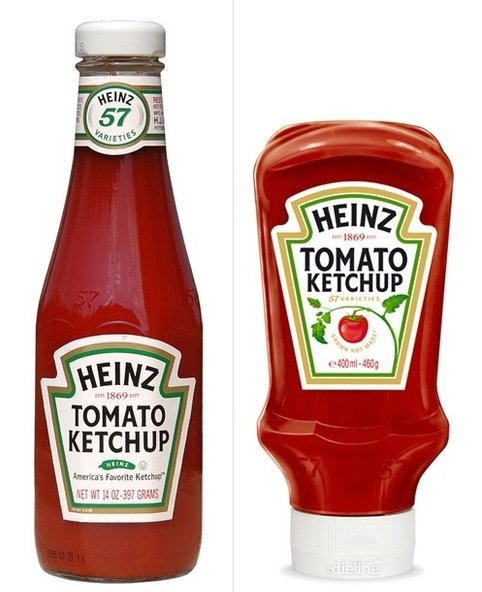
\includegraphics[scale=0.2]{figures/ketchup.png}
\caption{Heinz's tomato ketchup bottle before and after the innovation.}
\label{fig:heinz-ketchup-bottle}
\end{figure}
